\section{multiplexor de potencia}

    Para la selección de la batería que proporcionará la alimentación al agente
    robótico, asi como para la selección de la batería que se cargará se diseñó
    un multiplexor de potencia empleando transistores MOSFET canal P, en 
    configuración \textit{back to back} como se muestra en la figura \ref{fig:power_switch}.

    \begin{figure}[H]
        \centering
        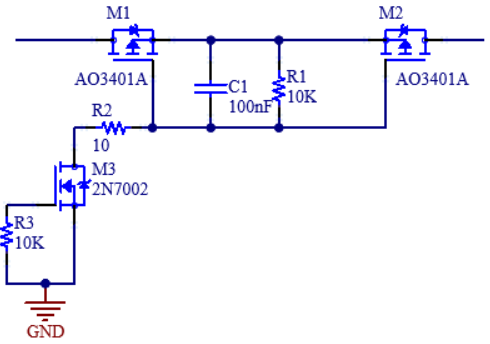
\includegraphics[scale=0.5]{imagenes/power_switch.png}
        \caption{Multiplexor de potencia}
        \label{fig:power_switch}
    \end{figure}

    En el conmutador de la figura \ref{fig:power_switch} se puede observar que se
    emplearon 2 transistores MOSFET caddnal P, de modelo AO3401, estos fueron
    seleccionados debido a que tienen una corriente de \textit{drain} máxima de
    $4\text{A}$, y una resistencia de \textit{drain} a \textit{source} de 
    $0.06\Omega$, lo cual permite que el multiplexor tenga una caída de tensión
    mínima cuando se encuentre en conducción, y un aumento de temperatura mínimo
    debido a la disipación de potencia \cite{a_AO3401}.

    La resistencia $R_1$ tiene como función asegurar que el voltaje 
    entre \textit{gate} y \textit{source} del transistor MOSFET sea de $0\text{V}$,
    cuando el transistor M3 no se encuentre en conducción, asegurando que 
    el conmutador no se encuentre en conducción cuando no se requiera. Los componentes 
    $R_2$ y $C_1$ tienen como función limitar la corriente drenada \textit{gate} de
    los transistores MOSFETs M1 y M2 de forma que se evite dañar los transistores
    cuando se realice el cambio de estado del conmutador, mientras que el propósito
    de la resistencia $R_3$ evitar que la terminal \textit{gate} del transistor
    M3 se encuentre en un estado flotante.

    Para el multiplexor encargado de seleccionar la batería que alimentará al
    agente robótico se utilizó un conmutador como el mostrado en la figura
    \ref{fig:power_switch}, en conjunto con el circuito interno posee el 
    Pololu 3pi+, que permite conectar y desconectar la batería NiMH integrada.

    Para el multiplexor encargado de seleccionar la batería que se cargará se
    emplearon 2 conmutadores como el mostrado en la figura \ref{fig:power_switch},
    el controlador que se describe en la sección \ref{sec:controlador} se encarga
    de seleccionar la batería que se cargará, y de seleccionar la batería que
    alimentará al agente robótico.

    Ambos multiplexores fueron diseñados para tener un funcionamiento manual, 
    es decir, que el microcontrolador será el encargado de seleccionar la batería
    que se cargará, y la batería que alimentará al agente robótico, no existiendo
    un comportamiento automático para la selección de las baterías.

    \subsection{Pruebas del conmutador de potencia}

    Para comprobar el correcto funcionamiento del conmutador de potencia diseñado
    se realizó el diseño de una placa de pruebas, la cual se muestra en la figura
    \ref{fig:power_switch_test}.

    \begin{figure}[H]
        \centering

        \begin{subfigure}{0.45\textwidth}
            \centering
            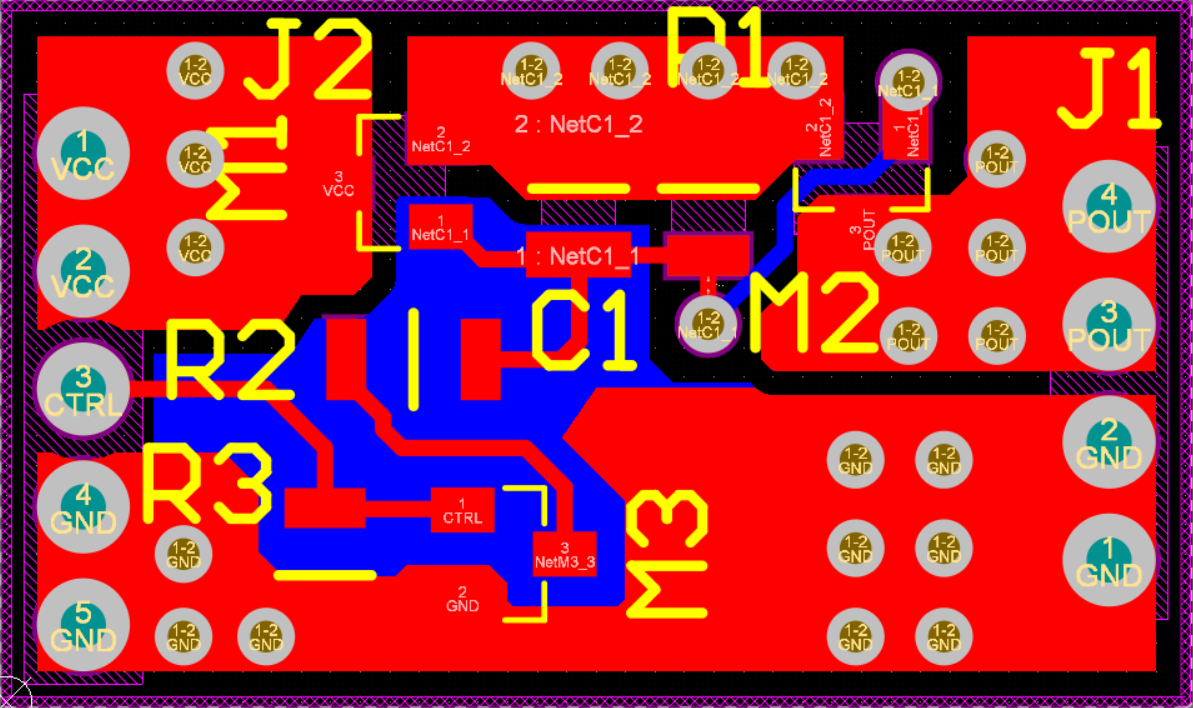
\includegraphics[scale=0.2]{imagenes/power_switch_test_top.png}
            \caption{Capa superior}
        \end{subfigure}
        \begin{subfigure}{0.45\textwidth}
            \centering
            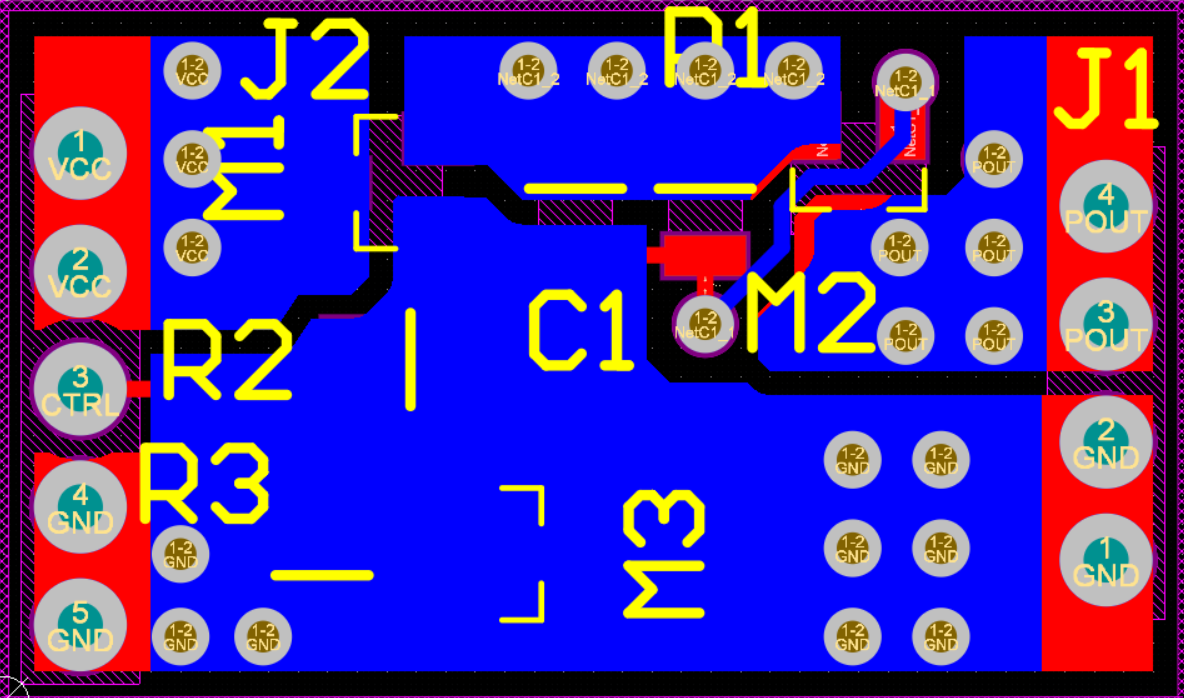
\includegraphics[scale=0.2]{imagenes/power_switch_test_bottom.png}
            \caption{Capa inferior}
        \end{subfigure}
        \vfill
        \begin{subfigure}{0.45\textwidth}
            \centering
            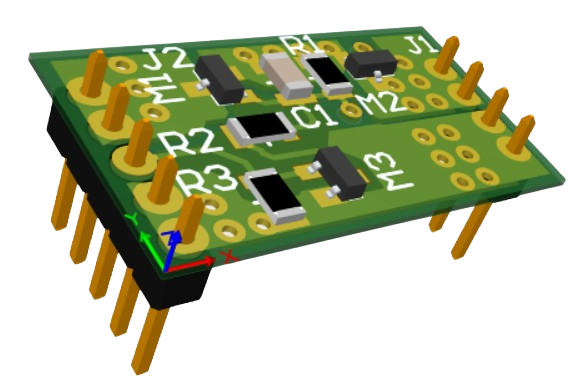
\includegraphics[scale=0.3]{imagenes/power_switch_test_3D.png}
            \caption{Vista 3D} 
        \end{subfigure}
        \begin{subfigure}{0.45\textwidth}
            \centering
            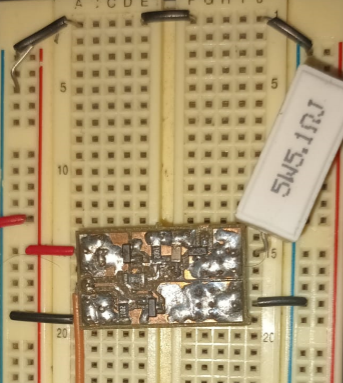
\includegraphics[scale=0.4]{imagenes/power_switch_test_asm.png}
            \caption{PCB ensamblada}
        \end{subfigure}

        \caption{Placa de pruebas del conmutador de potencia}
        \label{fig:power_switch_test}
    \end{figure}

        Al momento de realizar las pruebas el diseño del conmutador de potencia
        tuvo el comportamiento esperado, evitando el paso de corriente cuando
        el transistor MOSFET M3 no se encontraba en conducción, y permitiendo
        el paso de corriente cuando el transistor MOSFET M3 se encontraba en
        conducción. Adicionalmente se comprobó que la caída de tensión en el
        conmutador de potencia era de $0.12\Omega$ cuando se encontraba conduciendo
        una corriente de $3\text{A}$, y este no presentaba un aumento de temperatura
        significativo. En la figura \ref{fig:charger_anexo_mux} en el anexo \ref{sec:anexo_esquematico}
        se muestra el diseño final de los multiplexores de potencia.

        El diseño de este conmutador de potencia se encuentra dentro de los archivos
        adjuntos dentro de la carpeta nombrada como PCB\_Design dentro del proyecto
        de Altium nombrado como Pmos\_switch. 



    

    